\documentclass{article} 
\usepackage{geometry} 
\usepackage{longtable}
\usepackage{multicol} 
\usepackage[table]{xcolor}\geometry{a4paper, left=15mm, right=15mm, top=10mm} 
\usepackage[portuguese]{babel}
\usepackage[utf8]{inputenc}
\usepackage{graphicx}

\newcommand{\likert}{
	\begin{figure}[h!] \center
		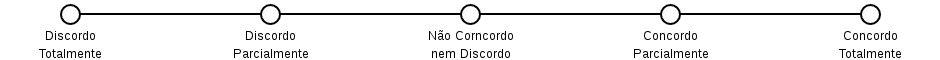
\includegraphics[width=0.8\textwidth]{Likert/likert.png} 
	\end{figure}
}


\newcommand{\likertA}{
	\begin{figure}[h!] \center
		
\includegraphics[width=0.8\textwidth]{Likert/likert-1.png} 
	\end{figure}
}



\newcommand{\likertB}{
	\begin{figure}[h!] \center
		
\includegraphics[width=0.8\textwidth]{Likert/likert-2.png} 
	\end{figure}
}



\newcommand{\resultsheader}[2] {
	\noindent \textbf{Consulta #1} -- \textbf{Técnica #2}
	 \vspace{0.5 cm} \\
	
}



%------------------------
\begin{document}
\pagestyle{empty}

\section*{Avaliação de extração de tópicos em atas de reuniões}
\vspace{1cm}


\subsection*{Apresentação}


Essa avaliação se refere a componentes de um sistema para consultas em atas de reunião. O objetivo dos sistema  é ajudar o usuário a fazer buscas por um assunto específico em uma coleção de atas de reunião. O Sistema deve receber uma consulta do usuário sobre um assunto e apresentar os trechos onde esse assunto é mencionado. As atas são documentos que não possuem um assunto principal, mas contém diversos assuntos registrados em um mesmo documento. Essa multiplicidade de assuntos das atas constitui um desafio para sistemas de consulta.

Inicialmente, o sistema analisa todas atas e divide o texto de cada ata em trechos que contêm um assunto principal e relativamente independente. Ou seja, os diversos assuntos tratados em uma ata são separados em trechos com um único assunto. Em seguida, utiliza-se técnicas de inteligência artificial para identificar trechos com assuntos relacionados e agrupá-los. Cada grupo contém trechos de atas diferentes mas com assuntos relacionados. Além disso, o sistema seleciona um conjunto de palavras que indicam o assunto do grupo. Assim, espera-se que o agrupamento de trechos com assuntos similares extraídos de diferentes documentos facilite a navegação e busca por assuntos na coleção de atas.

Para essa avaliação fez-se uma consulta ao sistema com os termos \textit{``compra de equipamentos''}. Três técnicas diferentes foram utilizadas para identificar trechos que tratam desse assunto e agrupá-los. Para cada um dos grupos apresentados, solicita-se que sejam respondidas algumas questões de forma a refletir a percepção do usuário quanto a qualidade dos resultados. 



\vspace{1cm}

Na imagem a seguir, é mostrada a tela principal do sistema com um campo para pesquisa na parte superior e abaixo os trechos pertencentes ao grupo selecionado. A esquerda estão os ícones seguidos de palavras que representam os grupos.


\begin{figure}[h!]
\center
	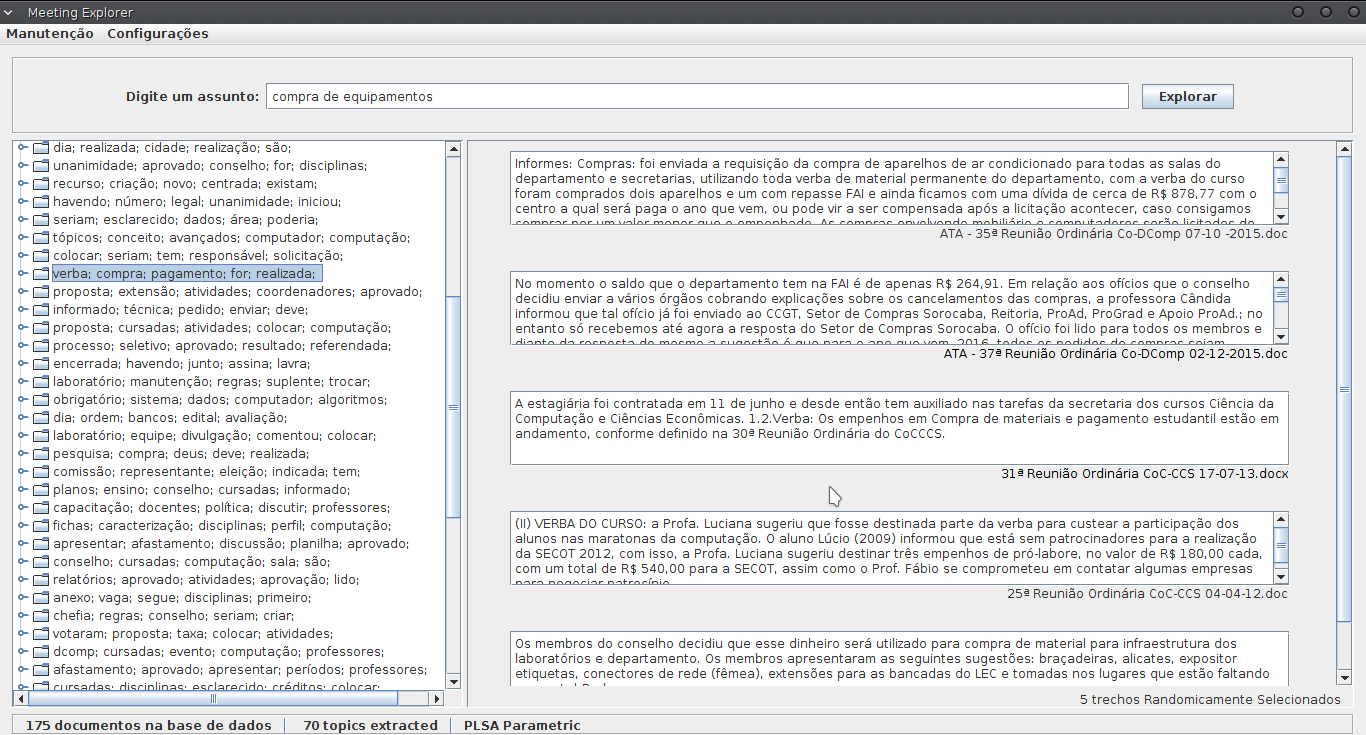
\includegraphics[width=1\textwidth]{prints/compra.png} 
\end{figure}







% --------------------


% --------------------

% Trata-se de um sistema para consultas em atas de reunião. O objetivo é ajudar o usuário a fazer buscas por um assunto específico em uma coleção de atas de reunião. O Sistema deve receber uma consulta do usuário sobre um assunto e apresentar os trechos onde esse assunto é mencionado. 

% Escolheu-se as atas por tratar-se de documentos que não possuem um assunto principal, mas contém diversos assuntos registrados em um mesmo documento. Essa multiplicidade de assuntos das atas constitui um desafio para sistemas de consulta e ao mesmo tempo motivou esse trabalho de mestrado.

% Para isso, visto a multiplicidade de assuntos uma mesma ata, o sistema inicialmente  analisa a coleção de atas e divide o texto de cada ata em trechos que contêm um assunto principal e relativamente independente. 
% Ou seja, os diversos assuntos tratados em uma ata são separados em trechos com um único assunto.
% Em seguida, utiliza-se técnicas de inteligência artificial para identificar trechos com assuntos relacionados e agrupá-los. Cada grupo contém trechos de atas diferentes mas com assuntos relacionados. Além disso, o sistema seleciona um conjunto de palavras descritoras que indicam o tópico do grupo. Nesse sistema, um grupo é formado por um conjunto de trechos e por um conjunto de palavras que o descreve.

% Assim, espera-se que o agrupamento de trechos com assuntos similares extraídos de diferentes documentos facilite a navegação e busca por assuntos na coleção de atas.

% Ao iniciar, o sistema apresenta os grupos anteriormente identificados os quais são representados por suas palavras descritoras. Ao selecionar um grupo, seus trechos são exibidos ao usuário para que possa verificar o que foi registrado sobre o assunto de cada grupo. 
% %
% O sistema também permite que o usuário faça consultas à coleção de atas por meio de um campo de pesquisa por palavras-chave. Nesse caso, o sistema  analisa as similaridades entre a consulta do usuário e os trechos extraídos das atas, bem como os grupos aos quais pertence. Então, apresenta os trechos ordenados pela relevância com a consulta do usuário. Para cada trecho é apresentado além do texto, um link para o arquivo original do qual foi extraído. Ao clicar sobre o texto de um trecho, seu grupo é destacado para que o usuário possa explorar outros trechos similares.


% Abaixo é mostrado a tela principal do sistema. A esquerda são apresentados os grupos com seus descritores e a direita os trechos atribuídos ao grupo selecionado. Acima está o campo para pesquisa.












% --> por que trechos? 

%Um trecho é representado por  texto  

%Com isso, espera-se que o agrupamento trechos de diferentes documentos, mas com assuntos similares, facilite a navegação e busca por assuntos na coleção de atas.


%Após realizar a busca, o sistema apresenta os trechos agrupados por tópicos, em que documentos com assuntos similares pertencem ao mesmo grupo. Ao selecionar um grupo, os trechos de atas são exibidos ao usuário.

%O sistema atribui um conjunto de palavras para cada grupo as quais servem para descrever o tópico do grupo.

%Cada grupo possui um conjunto de palavras 

%O sistema deve apresentar ao usuário os trechos de atas que melhor satisfazem a busca. 
 


%e documentos com assuntos diferentes ficam em gru


\newpage \resultsheader{1}{1} \noindent \textbf{Grupo de trechos:}

\begin{longtable}{|p{17.5cm}|}
\hline 
%1 & 
(III) COMPRAS COM VERBA DE MATERIAL DE CUSTEIO E PERMANENTE. (III.I) A professora AAA esclareceu que vamos continuar fazendo pedidos de compras e que chegaram novas demandas: compra de memória RAM para 32 máquinas (a pedido dos profs.

 \\ \hline 
%2 &
A professora AAA ficou responsável pela compra do material seguindo as sugestões dentro orçamento disponível.

 \\ \hline 
%3 &
Informes: O professor BBB informou que irá disponibilizar um link para abertura das solicitações de compras para 2015, e também que quando for realizada a reunião para distribuição das porcentagens da verba, irá solicitar o máximo possível para material permanente, visto que iremos precisar de verba permanente para equipar o prédio que será entregue o ano que vem.

 \\ \hline 
%4 &
(VII) DISCUSSÃO SOBRE A COMPRA DE MATERIAL PERMANENTE. (VII.I) Após discussão ficou acertado a compra de material e de informática e material para coffee break.

 \\ \hline 
%5 &
(IV) COMPRAS COM VERBA DE MATERIAL DE CUSTEIO E PERMANENTE (IV.I) A professora AAA forneceu os saldos parciais que ainda temos, em relação a capital para permanente temos em torno de R\$ 2918,00 reais o qual será utilizada para compra de um PC novo para secretaria do DComp-So, e quando for liberado a segunda parcela da verba de capital a intenção é que se compre câmeras para os laboratórios, nobreak para servidor e também que seja atendida as prioridades 3 e 4 dos professores que já constam em planilha. Os professores aprovaram a distribuição sugerida. Já em relação ao custeio embora o professor CCC não tenha atualizado a planilha, fizemos uma estimativa e acreditamos que temos em torno de 7 mil reais. Foi pedido para professores apresentarem suas demandas que foram a seguinte: 14 pro labores de 300 reais; 32 memórias RAM; divisória antirruídos para criar um espaço dentro da sala do ATLab onde está cluster, nessa sala ficaria o técnico DDD; placas para identificação das portas dos laboratórios; HD de 1Tb para o servidor do LaSID; 2 HDs de 2,5 polegadas de 500Gb e também 51 ventoinhas. A professora EEE apresentou a demanda para pagamento de diária, inscrição e passagem para apresentação de artigo em congresso. Foram aprovados os pro labores e demanda de infraestrutura, não sendo possível atender a demanda de ajuda de custo da professora FFF. Serão dados os encaminhamentos para aquisição dos materiais aprovados, tais compras serão requisitadas na medida em que a verba for liberada.

 \\ \hline 

\end{longtable} 



 
\newpage \resultsheader{1}{1}  \noindent \textbf{Questões:}
\newpage

\subsection*{Questões}


Com base na análise dos resultados anteriores, por favor informe sua concordância com a afirmações a seguir:


%responda as seguintes questões:



\begin{enumerate}

\item Todos os trechos apresentados compartilham um mesmo assunto.
\likert

\item Mais da metade dos trechos apresentados compartilham um mesmo assunto.
\likert

\item As palavas \textit{compra, material, verba, permanente e valor} resumem bem o assunto tratado nos trechos.
\likert

\item Existem trechos que não tratam de um único assunto.
\likert

\item Muitos trechos apresentados não tratam de um único assunto. 
\likert

\item Existem trechos incompletos e insuficientes para compreensão do assunto.
\likert

\item Muitos trechos são incompletos e insuficientes para compreensão do assunto.
\likert


%\item A navegação pelos tópicos ajuda a conduzir o usuário para o documento desejado.
%\likert

\end{enumerate}







%\begin{multicols}{5}
%
%\begin{itemize}
%\item Nada
%\item Pouco
%\item Razoável
%\item Bom
%\item Excelente
%\end{itemize}
%
%\end{multicols}
%
%\begin{multicols}{5}
%
%\begin{itemize}
%\item Discordo Totalmente
%\item Discordo Parcialmente
%\item Não Concordo nem Discordo
%\item Concordo Parcialmente
%\item Concordo Totalmente
%\end{itemize}
%


















\newpage \resultsheader{1}{2} \noindent \textbf{Grupo de trechos:}

\begin{longtable}{|p{17.5cm}|}
\hline 
%1 & 
Sobre as câmeras ele fez um orçamento informal de um sistema que atenda as nossas necessidades e foi passado um valor de aproximadamente cinco mil reais, já o ar condicionado ele ainda não tem o valor.

 \\ \hline 
%2 &
Informes: O professor AAA Informou que já foi estabelecida as regras de como será realizada a divisão do orçamento, porém ainda não temos nem ideia de qual será o valor.

 \\ \hline 
%3 &
Informes: A professora BBB informou que o ofício a respeito do processo de seleção do PIBIC será enviado, no entanto o tom do ofício foi suavizado, informou também que tem um valor em auxílio estudante que precisará liquidar ainda este ano, pois provavelmente ele não virará o ano por ser de 2015, sendo assim está aceitando sugestões para gastos do referido dinheiro com apoio a projetos de disciplinas no valor máximo de até 800 reais e o que sobrar será enviado como ajuda custos para SeCoT 2017.

 \\ \hline 
%4 &
(VI) DELIBERAÇÃO SOBRE ORÇAMENTO PARA 2015 - COMPRA DE MATERIAIS DA VERBA DE CUSTEIO. (VI.I) A Profa. BBB colocou que temos um total de R$ 25.339,71 e mais R$ 727,38 que foi destinado à pós, perfazendo um montante de R\$ 26.607,12 para serem gastos com custeio e aulas práticas, relatou que alguns itens já foram pedidos como toners para a impressora do departamento, cabos para a SeCoT, auxílio estudante para maratona e hoje iremos deliberar sobre a visita técnica pedida pela coordenação do curso de BCCS, o qual deve ficar entre 1500 a 2000 reais, pagamento de pró-labores para banca da pós-graduação (8 de aproximadamente 300 reais) e auxílio estudante para congresso também da pós-graduação (5 de 500 reais).

 \\ \hline 
%5 &
(V.I) O prof. CCC explicou que este ano foi a primeira vez que recebemos verbas para todas as alíneas, foram R\$2.365,52 para aulas práticas, R\$ 19.180,57 para custeio, R\$ 4.718,19 para material permanente e tínhamos segundo informações de São Carlos R\$ 1.386,72 na conta do repasse FAI. A verba de material permanente e repasse FAI, foi empenhada para compra de cadeiras para os laboratórios, R\$ 4.720,38 (verba material permanente) para compra 24 cadeiras e R\$ 1.180,10 (repasse FAI) para compra de mais 6 cadeiras. O professor CCC explicou que nossa maior verba era para custeio a qual poder ser usada com pró-labore, diárias, auxilio estudante e outros diversos empenhos inclusive auxilio ao pesquisador e também em serviços, o que não foi muito fácil, pois ainda não temos experiência neste tipo de requisição. A verba de custeio e de aula prática foi unificada e ficamos com o montante de R\$21.546,09, deste valor foi requisitado em material físico o total de R\$ 7.700,97, alguns itens foram requisitados em quantidade maior do que precisamos no momento para que tenhamos um estoque, pois não sabemos como será dividida a verba no próximo ano. Já com serviços o total empenhado foi de R\$ 1.888,49, sendo que R\$ 1.111,82 com assinatura do Dream Spark (valor do dia da requisição, o que pode variar pelo fato de ser em dólar), e com a Arte Gráfica o total de R\$ 776,67. Também empenhamos R\$ 1.200,00 para diárias, R\$ 528,00 para pró-labore e R\$ 300,00 com auxílio estudante. Em relação à compra da assinatura do Dream Spark, a compra já teria acontecido se a empresa não estivesse com pendência no INSS, o setor de compras entrou com a referida empresa e a mesma informou que tal pendência será resolvida até dia 05 de outubro, caso a compra concretize o Departamento de Administração irá arcar com a metade de valor por que eles estão interessados em utilizar o MS Visio. O professor CCC colocou que ainda temos um montante que gira em torno de R\$ 9.900,00 e dos quais mais ou menos R\$ 1.500,00 será gasto com a gráfica, R\$ 1.500,00 será permutado com o curso para compra de roteadores sem fio. Precisamos decidir onde empenharemos o restante, sendo que talvez tenhamos uma demanda de pagamento de passagens aéreas caso nossa equipe passe para a segunda fase da maratona de programação, (o total de 4 passagens). O conselho deliberou a favor de pagamento das passagens, porém sugeriu que as mesmas sejam pagas por meio de auxílio estudante, pois desta maneira o valor será bem menor. Aprovado. Também foi colocado o pedido da professora DDD para pagamento de taxa de inscrição no evento X IEEE International Conference on e Science, no valor de hoje de R\$ 1.725,00. Aprovado. O professor CCC apresentou mais um demanda de um serviço que seria a manutenção do servidor e do site do DComp e está avaliando a possibilidade de contratar a empresa Júnior para cuidar destes serviços, mas que ainda é preciso conversar com os alunos para acertar detalhes e expor melhor ideia e decidir na próxima reunião.

 \\ \hline 

\end{longtable} 





 	
\newpage  \resultsheader{1}{2} \noindent \textbf{Questões:}


\vspace{0.5 cm} 
\noindent Com base na análise dos trechos, responda as questões a seguir:
\vspace{0.5 cm} 



\begin{enumerate}



\item Os trechos apresentados compartilham um mesmo assunto?
% Nada; Pouco; Razoável, Bom; Excelente;
\likertB




\item As palavas \textit{verba, compra, pagamento, material e valor} resumem bem o assunto tratado nos trechos?
% Nada; Pouco; Razoável, Bom; Excelente;
\likertB




\item Existem trechos que não tratam de um único assunto?
% Nenhum; Poucos; Nem muito, nem pouco; Muitos; Todos
\likertA



\item Existem trechos incompletos e insuficientes para compreensão do assunto do trecho?
% Nenhum; Poucos; Nem muito, nem pouco; Muitos; Todos
\likertA



\end{enumerate}







%\begin{multicols}{5}
%
%\begin{itemize}
%\item Nada
%\item Pouco
%\item Razoável
%\item Bom
%\item Excelente
%\end{itemize}
%
%\end{multicols}
%
%\begin{multicols}{5}
%
%\begin{itemize}
%\item Discordo Totalmente
%\item Discordo Parcialmente
%\item Não Concordo nem Discordo
%\item Concordo Parcialmente
%\item Concordo Totalmente
%\end{itemize}
%


















\newpage \resultsheader{1}{3} \noindent \textbf{Grupo de trechos:}

\begin{longtable}{|p{17.5cm}|}
\hline 
%1 & 
Informes: Compras: foi enviada a requisição da compra de aparelhos de ar condicionado para todas as salas do departamento e secretarias, utilizando toda verba de material permanente do departamento, com a verba do curso foram comprados dois aparelhos e um com repasse FAI e ainda ficamos com uma dívida de cerca de R\$ 878,77 com o centro a qual será paga o ano que vem, ou pode vir a ser compensada após a licitação acontecer, caso consigamos comprar por um valor menor que o empenhado. As compras envolvendo mobiliário e computadores serão licitados de formas diferentes, será realizado um pedido para toda a universidade e serão comprados via ata, maiores informações de gastos verificar planilha anexa.

 \\ \hline 
%2 &
No momento o saldo que o departamento tem na FAI é de apenas R\$ 264,91. Em relação aos ofícios que o conselho decidiu enviar a vários órgãos cobrando explicações sobre os cancelamentos das compras, a professora AAA informou que tal ofício já foi enviado ao CCGT, Setor de Compras Sorocaba, Reitoria, ProAd, ProGrad e Apoio ProAd.; no entanto só recebemos até agora a resposta do Setor de Compras Sorocaba. O ofício foi lido para todos os membros e diante da resposta do mesmo a sugestão é que para o ano que vem, 2016, todos os pedidos de compras sejam colocados no sistema o mais rápido possível. Foi informado que a impressora do prédio já foi instalada e como o custo da impressão por esta impressora é bem mais baixo foi pedido a todos que as impressões sejam feitas na impressora em questão; porém a conexão por rede ainda não está funcionando, então para imprimir ainda é necessário o uso do pen drive. O professor BBB colocou que quando é cobrado do departamento o valor é referente ao papel e a impressão em si, no entanto não tem papel disponível e cada professor está levando seu próprio papel, sendo assim o departamento irá pagar duas vezes pelo mesmo papel. Diante deste problema iremos contatar o centro para que o mesmo nos apresente uma solução. Sobre os pagamentos de pró-labores para membros de banca da pós, foi informado que para este ano temos apenas mais dois, o qual está sendo pago com saldo de empenho de 2014 e como provavelmente este empenho não irá virar para 2016 a solução encontrada para não perder dinheiro foi elevar um pouco o valor do pagamento dos pró-labores. Foi realizado um pedido de inclusão de pauta pela professora CCC, a qual pede ajuda financeira do departamento para divulgação da calourada 2016, o pedido foi aceito. 

 \\ \hline 
%3 &
A estagiária foi contratada em 11 de junho e desde então tem auxiliado nas tarefas da secretaria dos cursos Ciência da Computação e Ciências Econômicas. 1.2.Verba: Os empenhos em Compra de materiais e pagamento estudantil estão em andamento, conforme definido na 30ª Reunião Ordinária do CoCCCS.

 \\ \hline 
%4 &
(II) VERBA DO CURSO: a Profa. DDD sugeriu que fosse destinada parte da verba para custear a participação dos alunos nas maratonas da computação. O aluno EEE (2009) informou que está sem patrocinadores para a realização da SECOT 2012, com isso, a Profa. DDD sugeriu destinar três empenhos de pró-labore, no valor de R$ 180,00 cada, com um total de R$ 540,00 para a SECOT, assim como o Prof. FFF se comprometeu em contatar algumas empresas para negociar patrocínio.

 \\ \hline 
%5 &
Os membros do conselho decidiu que esse dinheiro será utilizado para compra de material para infraestrutura dos laboratórios e departamento. Os membros apresentaram as seguintes sugestões: braçadeiras, alicates, expositor etiquetas, conectores de rede (fêmea), extensões para as bancadas do LEC e tomadas nos lugares que estão faltando para o LabRedes.

 \\ \hline 

\end{longtable} 




 	
\newpage  \resultsheader{1}{3}  \noindent \textbf{Questões:}
\newpage

\subsection*{Questões}


Com base na análise dos resultados anteriores, por favor informe sua concordância com a afirmações a seguir:


%responda as seguintes questões:



\begin{enumerate}

\item Todos os trechos apresentados compartilham um mesmo assunto.
\likert

\item Mais da metade dos trechos apresentados compartilham um mesmo assunto.
\likert

\item As palavas \textit{verba, compra, pagamento, valor e realizada} resumem bem o assunto tratado nos trechos.
\likert

\item Existem trechos que não tratam de um único assunto.
\likert

\item Muitos trechos apresentados não tratam de um único assunto. 
\likert

\item Existem trechos incompletos e insuficientes para compreensão do assunto.
\likert

\item Muitos trechos são incompletos e insuficientes para compreensão do assunto.
\likert


%\item A navegação pelos tópicos ajuda a conduzir o usuário para o documento desejado.
%\likert

\end{enumerate}







%\begin{multicols}{5}
%
%\begin{itemize}
%\item Nada
%\item Pouco
%\item Razoável
%\item Bom
%\item Excelente
%\end{itemize}
%
%\end{multicols}
%
%\begin{multicols}{5}
%
%\begin{itemize}
%\item Discordo Totalmente
%\item Discordo Parcialmente
%\item Não Concordo nem Discordo
%\item Concordo Parcialmente
%\item Concordo Totalmente
%\end{itemize}
%




















% 
\begin{longtable}{|p{17.5cm}|}
\hline 
%1 & 
(III) Aprovado a prorrogação de prazo para defesa de dissertação dos alunos Anderson Parra de Paula, orientado pelo Prof. Dr. Gustavo Maciel Dias Vieira, por 06 meses, André Breda Carneiro, orientado pela Prof. Dra. Cândida Nunes da Silva, por 06 meses, Diego Heitzmann Quintale, orientado pela Profa. Dra. Luciana Aparecida Martinez Zaina, por 06 meses, Elizeu Elieber Fachini, orientado pelo Prof. Dr. Gustavo Maciel Dias Vieira, por 06 meses, Marcel Popolin de Araújo Cunha, orientado pela Profa. Dra. Luciana Aparecida Martinez Zaina, por 06 meses; (IV) Homologado o relatório de defesa de dissertação do aluno Anderson Roque do Amaral, orientado pela Profa. Dra. Luciana Aparecida Martinez Zaina;

 \\ \hline 
%2 &
(III) aprovado o pedido de prorrogação de prazo para defesa de dissertação do aluno Tiago Pasqualini da Silva, orientado pelo Prof. Dr. Tiago Agostinho de Almeida por mais 06 meses com prazo final para setembro de 2015;

 \\ \hline 
%3 &
Aprovados os requerimentos de prorrogação de prazo para defesa de dissertação: Allan Castro Silva orientado pelo Prof. Dr. Fábio Luciano Verdi por mais 06 meses com prazo final para janeiro de 2016, Amauri Antunes filho orientado pelo Prof. Dr. Murillo Rodrigo Petrucelli Homem por mais 06 meses com prazo final para janeiro de 2016, Eline Faliane de Araújo Welter orientada pela Profa. Dra. Luciana Aparecida Martinez Zaina por mais 06 meses com prazo final para janeiro de 2016, Fabio Ruy orientado pelo Prof. Dr. Fabio Luciano Verdi por mais 06 meses com prazo final para janeiro de 2016, Jane Piantoni orientada pela Profa. Dra. Katti Faceli por mais 06 meses com prazo final para fevereiro de 2016, Johannes Von Lochter orientado pelo Prof. Dr. Tiago Agostinho de Almeida por mais 06 meses com prazo final para janeiro de 2016, Luiz Fernando Camargo Durello orientado pelo Prof. Dr. Murillo Rodrigo Petrucelli Homem por mais 06 meses com prazo final para janeiro de 2016, Thamires de Campos Luz orientada pelo Prof. Dr. Fabio Luciano Verdi por mais 06 meses com prazo final para janeiro de 2016; (IX) Homologado o relatório de defesa de dissertação do aluno Allan Vidal, orientado pelo Prof. Dr. Fabio Luciano Verdi, realizada em 08 de abril; Nada mais, Prof. Dr. Alexandre Alvaro Presidente desta Reunião Prof. Dr. Fábio Luciano Verdi Professor Adjunto Prof. Dr. José de Oliveira Guimarães Professor Associado Profa. Dra. Katti Faceli Professora Adjunta Johannes Von Lochter Representante Discente 87

 \\ \hline 
%4 &
Também foi discutida a situação de alunos que recebem a bolsa no decorrer do curso e apresentam o exame de defesa antes do término do prazo da bolsa. A duração da bolsa oferecida pela CAPES é de 24 meses e foi apresentada a proposta do aluno continuar com a bolsa caso solicite prorrogação do prazo de defesa da dissertação, desde que mantenha os requisitos descritos na norma 5 e não tenha nenhum aluno na lista de espera do ranking de bolsas elaborado pela Comissão de Bolsas de Estudos do PPGCCS. Foi decidido retirar os seguintes requisitos da norma 5: 1. b) Não ter completado 12 (doze) meses corridos a contar da data de sua primeira matrícula no curso de Mestrado, exceto no caso de renovação. 3. d) ultrapassar 24 (vinte e quatro) meses no Programa, ou 3. e) não tiver cumprido a Norma 6 sobre obrigatoriedade de solicitação de Bolsa FAPESP.

 \\ \hline 
%5 &
(II) Aprovado o pedido de agendamento de exame de defesa de dissertação do aluno Diego Heitzmann Quintale, orientado pela Profa. Dra. Luciana Aparecida Martinez Zaina, para o dia 24 de agosto, com banca formada pela Profa. Dra. Renata Pontin de Mattos Fortes, da USP e o Prof. Dr. Alexandre Alvaro; (III) Aprovados os pedidos de prorrogação de prazo para defesa de dissertação do aluno Eliezer Elieber Fachini orientado pelo Prof. Dr. Gustavo Maciel Dias Vieira por mais 06 meses com prazo final para fevereiro de 2016, André Breda Carneiro orientado pela Profa. Dra. Cândida Nunes da Silva por mais 06 meses com prazo final para fevereiro de 2016;

 \\ \hline 

\end{longtable} 



 

\vspace{0.5 cm} 
\noindent Com base na análise dos trechos, responda as questões a seguir:
\vspace{0.5 cm} 
% informe sua concordância com a afirmações a seguir:


\begin{enumerate}


\item Todos os trechos apresentados compartilham um mesmo assunto.
\likert





\item As palavas \textit{orientada, meses, defesa, prazo e dissertação} resumem bem o assunto tratado nos trechos.
\likert





\item Existem trechos que não tratam de um único assunto?
% Nenhum; Poucos; Nem muito, nem pouco; Muitos; Todos
\likertA



\item Existem trechos incompletos e insuficientes para compreensão do assunto do trecho?
% Nenhum; Poucos; Nem muito, nem pouco; Muitos; Todos
\likertA



\end{enumerate}







%\begin{multicols}{5}
%
%\begin{itemize}
%\item Nada
%\item Pouco
%\item Razoável
%\item Bom
%\item Excelente
%\end{itemize}
%
%\end{multicols}
%
%\begin{multicols}{5}
%
%\begin{itemize}
%\item Discordo Totalmente
%\item Discordo Parcialmente
%\item Não Concordo nem Discordo
%\item Concordo Parcialmente
%\item Concordo Totalmente
%\end{itemize}
%

















% 
\begin{longtable}{|p{17.5cm}|}
\hline 
%1 & 
(III) Aprovado o pedido de prorrogação de prazo para defesa de dissertação do aluno AAA orientado pelo Prof. Dr. BBB por mais 06 meses com prazo final para fevereiro de 2016, CCC orientada pela Profa. Dra. DDD por mais 06 meses com prazo final para fevereiro de 2016, EEE orientado pela Profa. Dra. FFF por mais 06 meses com prazo final para fevereiro de 2016;

 \\ \hline 
%2 &
(III) aprovado o pedido de prorrogação de prazo para defesa de dissertação do aluno AAA, orientado pelo Prof. Dr. BBB por mais 06 meses com prazo final para setembro de 2015;

 \\ \hline 
%3 &
(II) Aprovado o pedido de trancamento de matrícula da aluna AAA, orientada pelo Prof. Dr. BBB, para o segundo semestre de 2015;

 \\ \hline 
%4 &
(III) Aprovado a prorrogação de prazo para defesa de dissertação dos alunos AAA, orientado pelo Prof. Dr. BBB, por 06 meses, CCC, orientado pela Prof. Dra. DDD, por 06 meses, EEE, orientado pela Profa. Dra. FFF, por 06 meses, GGG, orientado pelo Prof. Dr. BBB, por 06 meses, HHH, orientado pela Profa. Dra. DDD, por 06 meses; (IV) Homologado o relatório de defesa de dissertação do aluno III, orientado pela Profa. Dra. DDD;

 \\ \hline 
%5 &
Aprovados os requerimentos de prorrogação de prazo para defesa de dissertação: AAA orientado pelo Prof. Dr. BBB por mais 06 meses com prazo final para janeiro de 2016, CCC orientado pelo Prof. Dr. DDD por mais 06 meses com prazo final para janeiro de 2016, EEE orientada pela Profa. Dra. FFF por mais 06 meses com prazo final para janeiro de 2016, GGG orientado pelo Prof. Dr. HHH por mais 06 meses com prazo final para janeiro de 2016, III orientada pela Profa. Dra. JJJ por mais 06 meses com prazo final para fevereiro de 2016, KKK orientado pelo Prof. Dr. LLL por mais 06 meses com prazo final para janeiro de 2016, MMM orientado pelo Prof. Dr. NNN por mais 06 meses com prazo final para janeiro de 2016, OOO orientada pelo Prof. Dr. PPP por mais 06 meses com prazo final para janeiro de 2016; (IX) Homologado o relatório de defesa de dissertação do aluno QQQ, orientado pelo Prof. Dr. DDD, realizada em 08 de abril; Nada mais, Prof. Dr. DDD Presidente desta Reunião Prof. Dr. BBB Professor Adjunto Prof. Dr. HHH Professor Associado Profa. Dra. JJJ Professora Adjunta GGG Representante Discente 87

 \\ \hline 

\end{longtable} 





%Após realizar a busca por palavras chave, o usuário selecionou o grupo ao qual pertence o trecho 5 dos resultados anteriores.
%Abaixo estão relacionados os 10 primeiros trechos que o sistema apresentou após essa ação bem como os descritores desse grupo.
% é possível analisar o grupo ao qual cada trecho pertence para encontrar outros resultados similares. 



%\begin{longtable}{|p{17.6cm}|}
%\hline 
%\textbf{Descritores:}  planos, ensino, sistema, disciplinas, algoritmos\\ 
%\hline 
%\end{longtable} 
 	\newpage

\subsection*{Questões}


Com base na análise dos resultados anteriores, por favor informe sua concordância com a afirmações a seguir:


%responda as seguintes questões:



\begin{enumerate}

\item Todos os trechos apresentados compartilham um mesmo assunto.
\likert

\item Mais da metade dos trechos apresentados compartilham um mesmo assunto.
\likert

\item As palavas \textit{aprovado, defesa, pedido, dissertação e orientada} resumem bem o assunto tratado nos trechos.
\likert

\item Existem trechos que não tratam de um único assunto.
\likert

\item Muitos trechos apresentados não tratam de um único assunto. 
\likert

\item Existem trechos incompletos e insuficientes para compreensão do assunto.
\likert

\item Muitos trechos são incompletos e insuficientes para compreensão do assunto.
\likert


%\item A navegação pelos tópicos ajuda a conduzir o usuário para o documento desejado.
%\likert

\end{enumerate}







%\begin{multicols}{5}
%
%\begin{itemize}
%\item Nada
%\item Pouco
%\item Razoável
%\item Bom
%\item Excelente
%\end{itemize}
%
%\end{multicols}
%
%\begin{multicols}{5}
%
%\begin{itemize}
%\item Discordo Totalmente
%\item Discordo Parcialmente
%\item Não Concordo nem Discordo
%\item Concordo Parcialmente
%\item Concordo Totalmente
%\end{itemize}
%

















% 
\begin{longtable}{|p{17.5cm}|}
\hline 
%1 & 
(III) Aprovado o pedido de prorrogação de prazo para defesa de dissertação do aluno AAA orientado pelo Prof. Dr. BBB por mais 06 meses com prazo final para fevereiro de 2016, CCC orientada pela Profa. Dra. DDD por mais 06 meses com prazo final para fevereiro de 2016, EEE orientado pela Profa. Dra. DDD por mais 06 meses com prazo final para fevereiro de 2016;

 \\ \hline 
%2 &
(II) Aprovado o pedido de prorrogação de prazo para defesa de dissertação do aluno AAA por mais 06 meses com prazo final para fevereiro de 2016. A partir de agora o formulário para solicitação de prorrogação de prazo para defesa de dissertação possui a opção de prorrogar a bolsa de estudos: No último mês de vigência da bolsa de estudos, será consultada a lista de espera por bolsas do PPGCCS. A solicitação de prorrogação de bolsa só será analisada caso não existam candidatos na fila de espera e se a vigência da bolsa não tiver atingido 24 meses. Neste caso, se a prorrogação for atendida, o novo prazo de vigência da bolsa será estendido para coincidir com a data prevista da defesa ou até que se complete 24 meses de bolsa (o que ocorrer primeiro);

 \\ \hline 
%3 &
(III) aprovado o pedido de prorrogação de prazo para defesa de dissertação do aluno AAA, orientado pelo Prof. Dr. BBB por mais 06 meses com prazo final para setembro de 2015;

 \\ \hline 
%4 &
Comunicação da Presidência: a presidente do Conselho, Profa. Dra. AAA comunicou que: a Coordenação do curso assumirá a Secot em 2015 ; foi agendado para 25/11/2014 o pregão para a compra dos roteadores; foi feita a distribuição das salas do novo prédio do CCGT, que terá sala para os professores, salas de estudo, auditório, sala para as secretarias (coordenações de cursos de graduação, pós-graduação e departamentos); no dia 29/11/2014, os alunos inscritos no ENADE foram convocados para uma reunião com a profª. CCC, pró-reitora de graduação adjunta, que enfatizou sobre a importância da participação dos alunos na prova marcada para o dia 23/11/2014, e avisou que o aluno concluinte que não fizer a prova ficará em débito com o MEC e não terá seu diploma impresso; a Comissão Própria de Avaliação (CPA) da UFSCAR fará uma avaliação interna dos cursos que participam do ENADE este ano e conta com a participação dos docentes e discentes deste curso. 2. Comunicação dos Conselheiros - a professora AAA comunicou que em 07/11/2014 começa a final da XIX Maratona de Programação, que acontecerá em Fortaleza.

 \\ \hline 
%5 &
Divulgação da lista de candidatos: 25 de maio; Prazo para recursos da lista de candidatos, 26 de maio até às 12 horas; Divulgação da lista final de candidatos: 26/5;

 \\ \hline 

\end{longtable} 




 	\newpage

\subsection*{Questões}


Com base na análise dos resultados anteriores, por favor informe sua concordância com a afirmações a seguir:


%responda as seguintes questões:



\begin{enumerate}

\item Todos os trechos apresentados compartilham um mesmo assunto.
\likert

\item Mais da metade dos trechos apresentados compartilham um mesmo assunto.
\likert

\item As palavas \textit{orientada, prazo, bolsa, meses e defesa} resumem bem o assunto tratado nos trechos.
\likert

\item Existem trechos que não tratam de um único assunto.
\likert

\item Muitos trechos apresentados não tratam de um único assunto. 
\likert

\item Existem trechos incompletos e insuficientes para compreensão do assunto.
\likert

\item Muitos trechos são incompletos e insuficientes para compreensão do assunto.
\likert


%\item A navegação pelos tópicos ajuda a conduzir o usuário para o documento desejado.
%\likert

\end{enumerate}







%\begin{multicols}{5}
%
%\begin{itemize}
%\item Nada
%\item Pouco
%\item Razoável
%\item Bom
%\item Excelente
%\end{itemize}
%
%\end{multicols}
%
%\begin{multicols}{5}
%
%\begin{itemize}
%\item Discordo Totalmente
%\item Discordo Parcialmente
%\item Não Concordo nem Discordo
%\item Concordo Parcialmente
%\item Concordo Totalmente
%\end{itemize}
%




















\end{document}




